\documentclass[a4paper,oneside,10pt,DIV12,headsepline,footexclude,headexclude]{scrartcl}

%% Normal LaTeX or pdfLaTeX? %%%%%%%%%%%%%%%%%%%%%%%%%%%%%%%%
%% ==> The new if-Command "\ifpdf" will be used at some
%% ==> places to ensure the compatibility between
%% ==> LaTeX and pdfLaTeX.
\newif\ifpdf
\ifx\pdfoutput\undefined
	\pdffalse              %%normal LaTeX is executed
\else
	\pdfoutput=1
	\pdftrue               %%pdfLaTeX is executed
\fi

%% Packages for Graphics & Figures %%%%%%%%%%%%%%%%%%%%%%%%%%
\ifpdf %%Inclusion of graphics via \includegraphics{file}
	\usepackage[pdftex]{graphicx} %%graphics in pdfLaTeX
\else
	\usepackage[dvips]{graphicx} %%graphics and normal LaTeX
\fi
\graphicspath{{fig/}}

%% Fonts for pdfLaTeX %%%%%%%%%%%%%%%%%%%%%%%%%%%%%%%%%%%%%%%
%% ==> Only needed, if cm-super-fonts are not installed
%%\ifpdf
%	%\usepackage{ae}       %%Use only just one of these packages:
%	%\usepackage{zefonts}  %%depends on your installation.
%%\else
%	%%Normal LaTeX - no special packages for fonts required
%%\fi

\renewcommand{\rmdefault}{pbk} % bookman
\renewcommand{\sfdefault}{phv} % helvetica (avantgarde = pag)
\renewcommand{\ttdefault}{pcr} % courier
\renewcommand{\familydefault}{phv}

%\usepackage{cmbright}  % computer modern bright - not for pdf


\areaset{16cm}{24cm}
\addtolength{\topskip}{0.5cm}


% texttt hyphenation
\newcommand{\origttfamily}{}
\let\origttfamily=\ttfamily
\renewcommand{\ttfamily}{\origttfamily \hyphenchar\font=`\-}


\let\ifpdf\relax

%\usepackage[T1]{fontenc}
%\usepackage[latin1]{inputenc}
\usepackage{tikz}
\usepackage[utf8]{inputenc}
\usepackage{array}
\usepackage{float}
%\usepackage{paralist}
\usepackage{color}
\usepackage{colortbl}

\usepackage{listings}
\lstset{language=Java,basicstyle=\ttfamily\small,tabsize=2}


%% Line Spacing %%%%%%%%%%%%%%%%%%%%%%%%%%%%%%%%%%%%%%%%%%%%%
%\usepackage{setspace}
%\singlespacing        %% 1-spacing (default)
%\onehalfspacing       %% 1,5-spacing
%\doublespacing        %% 2-spacing

\linespread{1.05}
\addtolength{\parskip}{0.175\baselineskip}

\widowpenalty = 10000
\clubpenalty = 10000


%%%%%%%%%%%%%%%%%%%%%%%%%%%%%%%%%%%%%%%%%%%%%%%%%%%%%%%%%%%%%
%% DOCUMENT
%%%%%%%%%%%%%%%%%%%%%%%%%%%%%%%%%%%%%%%%%%%%%%%%%%%%%%%%%%%%%
\begin{document}

%% File Extensions of Graphics %%%%%%%%%%%%%%%%%%%%%%%%%%%%%%
%% ==> This enables you to omit the file extension of a graphic.
%% ==> "\includegraphics{title.eps}" becomes "\includegraphics{title}".
%% ==> If you create 2 graphics with same content (but different file types)
%% ==> "title.eps" and "title.pdf", only the file processable by
%% ==> your compiler will be used.
%% ==> pdfLaTeX uses "title.pdf". LaTeX uses "title.eps".
\ifpdf
	\DeclareGraphicsExtensions{.pdf,.jpg,.png}
\else
	\DeclareGraphicsExtensions{.eps}
\fi


\pagestyle{plain} %Now display headings: headings / fancy / ...

\title{\Large People Tracking}

\author{\large Constantin Schieber, 1228774, Technische Universitaet Wien}
%\date{} %%If commented, the current date is used.

\maketitle

\begin{abstract}
This paper summarizes and discusses current research in the field of 
people tracking.
First, the established hardware, its limitations and
possible combinations are presented. Second, the widely used Robotic
Operating System (ROS) and its features of a distributed approach are introduced.\\
Then a detailed discussion on tracking of people with RGB-D hardware in a ground
plane, indoor enviroment is done.
The obtained results promise a good foundation for future work.

\end{abstract}

\begin{section}{Introduction and Problem Statement}

%%FIRST
%Highlighting the importance of the topic, and/or
Detection and tracking of people is an important feature for many applications.
Especially in the sphere of mobile robotics - where safe interactions with
people are a basic requirement in any situation. But particularly in mobile
applications there are several limiting constraints as e.g. computing power,
field of view and time for decision making.\\
%Making general statements about the topic, and/or
With the improvement of hardware in the relevant technology sector (e.g. RGB-D cameras, 
Laser, Thermal View) the number of papers focusing on this topic increased too.\\
%Presenting an overview on current research on the subject.
Reliable tracking of multiple persons that are partially blocked is 
possible with RGB-D camera networks that are set up prior to usage in a room in
combinations with solutions like OpenPTrack ~\cite{munaro2014openptrack}.\\
The same principles and hardware can be used in mobile applications as in 
~\cite{munaro2012tracking}. A different approach is tracking by a combination of 
laser and thermal view  as in ~\cite{7139259}.\\

%%THIRD
%Stating the intent of your study,
This paper intents to highlight the currently used hardware, the Robot Operating
System (ROS) as a framework for the hardware and the basic idea of currently
used detection and tracking approaches. 
\newpage

\begin{subsection}{Used Hardware}
RGB Sensors won't be used on their own as they only deliver depth information
when used in a stereo image approach and are usually combined with a depth sensor. 
This combination provides good enough performance to enable resource efficient 
and prompt computation of the environment.\\
Laser sensors provide accurate depth readings and a wide field of view but therefore
depend on body features like legs for proper detection. They are well suited for
close range following and tracking tasks as they provide accurate readings on close
distances, in contrast to Depth Sensors ~\cite{7139259}.\\
Thermal sensors provide readings that can be interpreted accurately when the 
targets of interest have a distinct temperature from the rest of the environment ~\cite{ciric2013computationally}.\\
Sonar sensors require an active counterpart on the person that is to be tracked. 
Therefore it is only suitable for tracking of single persons but works well
in the outside.\\


The following Table \ref{tab:title} shows a set of the currently utilized hardware for detection
and / or tracking of people.\\
\begin{minipage}{\linewidth}
\bigskip
\centering
\begin{tabular}{l | c c c c}
    \hline
    Sensor-type  & Depth Information & Works in sunlight & Requires Active Tag &    \\
    \hline
    RGB         & Bad   & Yes       & No &   \\
    Depth       & Good  & No        & No &   \\
    Laser       & Good  & Yes       & No &   \\
    Thermal     & Bad   & Yes       & No &   \\
    Sonar       & Good  & Yes       & Yes &  \\
    \hline
\end{tabular}\par
\captionof{table}{Summary of common sensor functionality} \label{tab:title} 
\end{minipage}
\end{subsection}

\begin{subsection}{Robotic Operating System}
Most mobile robotic applications work with the same underlying software framework, the Robotic 
Operating System (ROS). This framework provides operating system like features,
and can be used in a distributed heterogeneous group of nodes, enabling reliable 
communication between different sensors, actors and processing units.\\
The ROS Project is open source and provides a package system that makes sharing
of highly specialized solutions between different working groups easy.
Integration of these solutions is easy as only a communication between the new
node and the existing nodes has to be established. \\
Figure \ref{fig:ros} below shows the node based approach ROS takes.
By providing communication between the different nodes it is even possible to 
stream data to an extern PC for further analysis and processing. All Nodes are
registered at a master node and can then communicate directly with each other
as needed ~\cite{RosDoku}\\

\begin{center}
\begin{figure}[h]
\centering
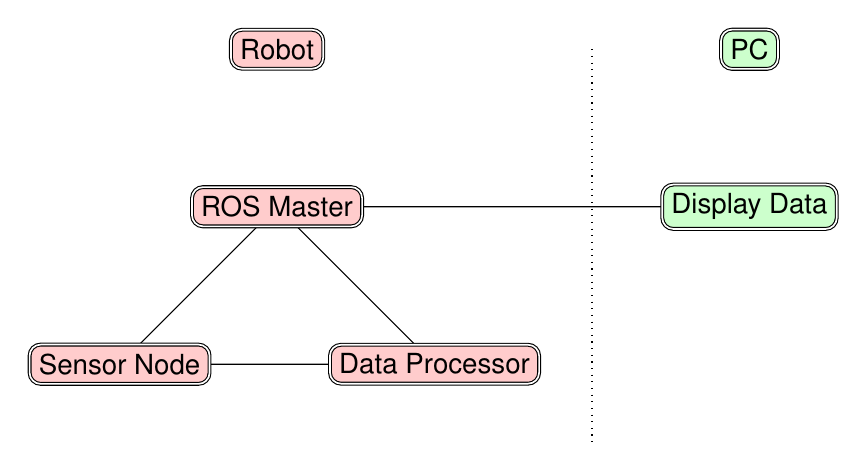
\begin{tikzpicture}[]
\draw[solid]
(0,0) node[fill=red!20,draw,double,rounded corners] {ROS Master}
-- (-2,-2)node[fill=red!20,draw,double,rounded corners] {Sensor Node}
(0,0) -- (2,-2)node[fill=red!20,draw,double,rounded corners] {Data Processor}
(-1,-2) -- (2,-2)
(0,0) -- (6, 0)node[fill=green!20,draw,double,rounded corners] {Display Data}
(6, 2)node[fill=green!20,draw,double,rounded corners] {PC}
(0, 2)node[fill=red!20,draw,double,rounded corners] {Robot};
\draw[dotted] (4, 2) -- (4,-3);
\end{tikzpicture}
\caption{Typical distribution of task on nodes in ROS}
\label{fig:ros}
\end{figure}
\end{center}
\end{subsection}

%%SECOND
%Formulating a research question or problem, and/or

%Outlining the key characteristics of your study,
%Describing important results, and
%Giving a brief overview of the structure of the paper.
\end{section}
\begin{section}{Methodology}
%How was the data collected or generated?
Data for this paper was obtained from the respective cited paper.\\
The cited papers themselves use a formal approach but omit predicted outcomes as
testing in experiments is inevitable due to extern conditions that can't be modeled.\\
A typical experiment for tracking / detection will focus on following key points, 
as these indicate the quality of the solution very well: valid assignments, 
ID switches ($ID$), misses ($Miss$)  and false positives ($FP$).\\
These values can be aggregated together to evaluate the \textit{multi-object accuracy tracking (MOTA)} score,
as described in ~\cite{7139259} by the formula: 
\begin{center}
$MOTA = 1 - \frac{\sum_{k}(ID_{k}+Miss_{k}+FP_{k})}{\sum_{k}g_{k}}$
\end{center}
$g_{k}$ represents the ground truth annotations and $k$ is the time. This weighs
all errors with the same weight, which may shed a wrong light on the application
and its intended use case scenario.\\
To quantify how precise a target is tracked if it is properly tracked over a given
time frame the \textit{muli-object tracking precision (MOTP)} is introduced ~\cite{7139259}.
$c_{k}$ is the number of matchings between estimated people positions and ground truth values.
It is put into proportion with $d_{k}^{i}$, which describes the distance between the \textit{i}th match
as follows:
\begin{center}
$MOTP = \frac{\sum_{i,k}d_{k}^{i}}{\sum_{k}c_{k}}$
\end{center}

%And, how was it analyzed?
%Written in past tense
\end{section}
\begin{section}{Major Findings of the Papers}
\begin{subsection}{Tracking with RGB-D Data}
The paper ~\cite{munaro2012tracking} discusses tracking of people with the help
of RGB-D Data in a mobile platform.\\
Figure \ref{fig:processSteps} shows the steps that are needed to be performed for
yielding a close to real time performance (approx. 26 Images per Second).
\begin{figure}[h]
\centering
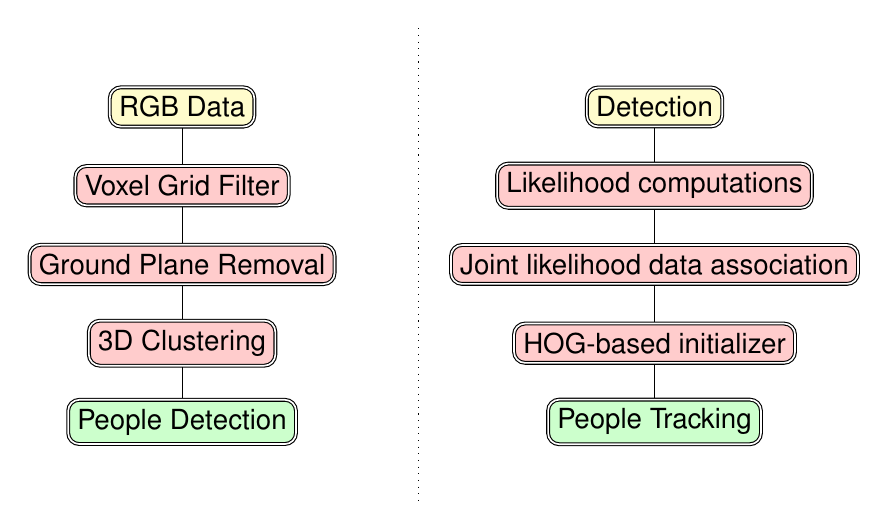
\begin{tikzpicture}[]
\draw[solid]
(0,0) node[fill=yellow!20,draw,double,rounded corners] {RGB Data}
-- (0,-1)node[fill=red!20,draw,double,rounded corners] {Voxel Grid Filter}
-- (0,-2)node[fill=red!20,draw,double,rounded corners] {Ground Plane Removal}
-- (0,-3)node[fill=red!20,draw,double,rounded corners] {3D Clustering}
-- (0,-4)node[fill=green!20,draw,double,rounded corners] {People Detection};
\draw[solid]
(6,0) node[fill=yellow!20,draw,double,rounded corners] {Detection}
-- (6,-1)node[fill=red!20,draw,double,rounded corners] {Likelihood computations}
-- (6,-2)node[fill=red!20,draw,double,rounded corners] {Joint likelihood data association}
-- (6,-3)node[fill=red!20,draw,double,rounded corners] {HOG-based initializer}
-- (6,-4)node[fill=green!20,draw,double,rounded corners] {People Tracking};
\draw[dotted] (3, 1) -- (3,-5);
\end{tikzpicture}
\caption{Process of detecting and tracking a person (from ~\cite{munaro2012tracking}) }
\label{fig:processSteps}
\end{figure}
\begin{subsubsection}{Voxel Grid Filter and Ground Plane Removal}
To reduce the amount of data that needs to be processed a filter is applied on
the point cloud that the sensor delivers. This is done by dividing the frame
into voxels (volumetric pixel) of 0.06m. All points in a voxel are then approximated
with coordinates of their centroid.\\
Since it can be assumed that people stand on the ground the ground plane can also
be removed from the already shrinked point cloud.
\end{subsubsection}
\begin{subsubsection}{3D Clustering}
After removing the ground plane, distinct people should no longer be connected to
each other and the 3D points could be clustered on that basis. To overcome problems
like splitting one person into multiple clusters if it is partially occluded or 
merging multiple persons into the same cluster due to being to close to each other
another feature of the human body is considered: The head. As the head should be
the highest part of any human and also is the one to be least likely occluded it
can be used as a metric for splitting clusters correctly. Local maxima in the
clusters are determined and, assuming that 0.3m is the intimate distance between
two individual, all points in that distance are associated with the cluster of 
the local maxima. If clusters have too few points or don't match a certain height
they are discarded.\\
A HOG (Histogram of Oriented Gradients, Matlab Toolbox) Detector is then applied on the parts
of the RGB Image where Subclusters were detected to further reduce the chance
for mismatches.
\end{subsubsection}
\begin{subsubsection}{Tracking}
Tracking is composed of three components: Motion of the tracked object, color
appearance and people detection confidence.\\
A maximization of a joint likelihood is performed between these three components 
in order to solve the data association problem.
\paragraph{Color Appearance}\mbox{}\\
The challenge in using the color appearance of an object is to select relevant
colors of this object that make it distinct to other tracked objects in the same
environment. The solution reflects this and uses an online classifier based on Adaboost 
for weighing the color appearance. A color histogram is computed from the RGB Image
of the current detection (that already has an associated track). \\
Weak classifiers in the histogram are pooled by randomized parallelepides, the 
sum of histogram elements within this parallelepide is the feature value.\\
To improve the training process not only random negative examples are selected
but also histograms of detections that are not associated with the current track.
This improves the distinction between different tracks further by increasing
the difference in confidence between the currently observed and other tracks.
\paragraph{Detection and Motion}\mbox{}\\
The velocity of the tracked object is determined by an Unscented Kalman filter to predict 
a future track. A constant velocity model was chosen, as it yields good results
for full occlusion scenarios.\\
The Mahalanobis distance (The distance between two points in a multidimensional vector space)
between the current detected position and the and the predicted state of the track
is calculated, based on the velocity of the object. 
\end{subsubsection}
\begin{subsection}{Experiments}
The paper chose three different test scenarios to validate its setup and
evaluated them with the \textit{MOTA} and \textit{MOTP} metrics explained in the
methodology section. The videos that were tested were manually annotated with 
ground truth values.\\
The results are good, with \textit{MOTA} values of over 80\% and \textit{MOTP} values over
90\% for every scenario.
The three test stages were designed as follows:
\begin{itemize}
\item No obstacles, linear trajectories of human objects
\item No obstacles, more difficult trajectories and interaction between human objects
\item Obstacles, more difficult trajectories and interaction between human objects 
\end{itemize}
A second test was performed on a publicly available RGB-D Dataset that was 
recorded with 3 Kinect Sensors. This dataset is fully annotated and allows for 
performance comparison between different approaches that use RGB-D sensor data
as input. The performance is again good, but \textit{MOTA} values were down to 
roughly 70\%, compared to 78\% from the algorithm the paper chose to benchmark against ~\cite{luber2011people}.
The number of ID Switches and False Positives were lower than the ones in the 
other approach. 
\end{subsection}
\end{subsection}

\end{section}

\begin{section}{Critical Reflection}
The paper shows an robust detection and tracking algorithm that performs well
in the concluded experiments.\\
Nothing is said on the outdoor performance though, which could suffer due to the
use of RGB-D sensors as main source for depth perception. Stereo Cameras replace
the RGB-D sensors in such a scenario but may result in excessive use of computing
power. The approach is also designed for working well in even terrain by removing
the ground plane from the voxel grid. This will be another point of failure for
a good outdoor performance. \\ 
This is also indicated in the second experiment where the \textit{MOTA} value
mainly decreases due to the presence of many people on stairs in the dataset. \\
More experiments in this direction would be desirable.

\end{section}
\begin{section}{Conclusion}
The paper shows a very fast and resource efficient approach that is suitable for
a wide variety of scenarios (static and mobile, different hardware).
Due to the assumpation that people move on an even pane and the subclustering approach
enables the algorithm to work well with people close to each other or people that
are close to the background.\\
Due to the use of ROS multiple sensors sources can be utilized and processed in an
multi-threaded way.
New test scenarios emerge for the future, e.g. using a network of robots for
imaging and computing the enviroment.

\end{section}


\bibliography{references}
\bibliographystyle{IEEEtran}
\end{document}
